\section{Pre-telegrapher wormhole baseline}
\label{app:pre-telegrapher}
This appendix preserves the failed lapse-front experiment that motivated the relaxation gauge in Sec.~\ref{sec:telegraph}. It uses the genuine wormhole construction of Sec.~\ref{sec:wormhole}, before the telegrapher lapse addition. Figure~\ref{fig:front} is historical baseline evidence and does not describe the selected telegrapher candidate.

For $M=1/3$ and $\nu=1$, the modified logarithmic source still produces a sharp inward-moving front. At $t=2.5$, the physical-lapse gradient near $r=0.119$ increases from $22.86$ to $40.65$ to $76.92$ as $N$ increases from $513$ to $1025$ to $2049$. The trace develops a narrow negative spike, and local Hamiltonian maxima increase from $0.409$ to $0.654$ to $0.974$ (Fig.~\ref{fig:front}). The front subsequently moves inward. These data rule out a smooth, resolved convergence interpretation of that trial. They support a gauge-steepening diagnosis, but do not prove a gauge-shock theorem for this spherical, nonlocal-shift system. Results for simpler slicing systems\cite{Alcubierre2005,BaumgarteHilditch2022} motivate this interpretation without establishing it here.

\begin{figure*}[tp]
 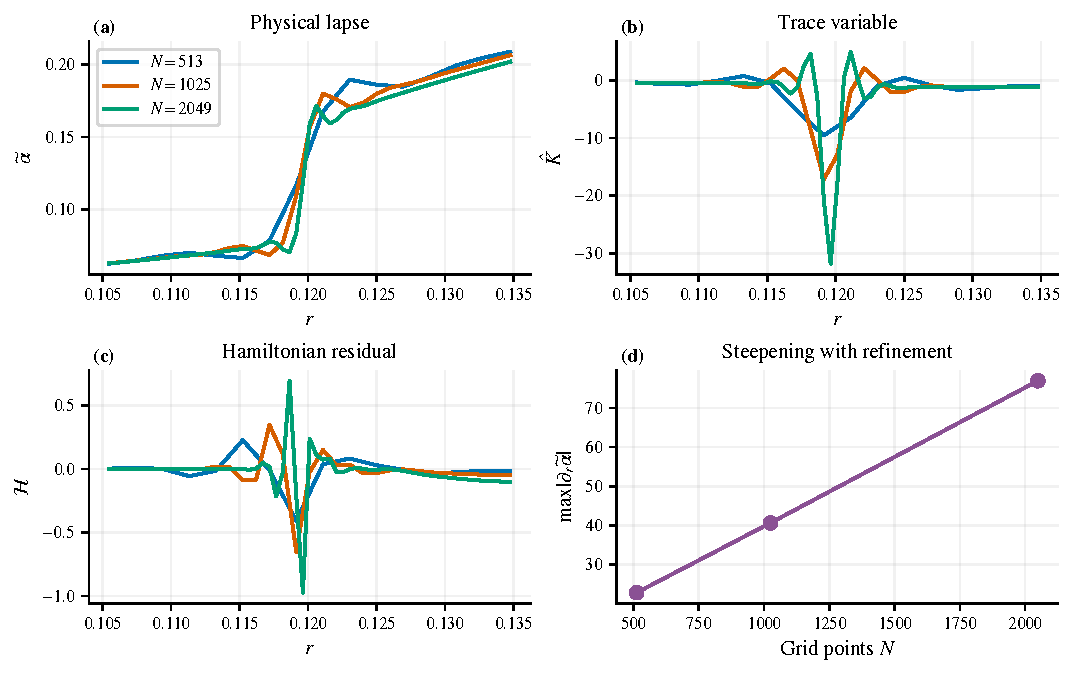
\includegraphics[width=\textwidth]{wormhole_front}
 \caption{Pre-telegrapher baseline: failed $\nu=1$ wormhole trial with the modified logarithmic source, shown at the exact saved time $t=2.5$. The physical lapse steepens, $\Kh$ develops a narrow spike, and the local Hamiltonian error grows under refinement. The gradient diagnostic in (d) uses second-order differentiation of saved profiles; it is not the evolution stencil. This is evidence of unresolved steepening, not a proof of a continuum shock.}
 \label{fig:front}
\end{figure*}
